%\stepcounter{unitday}

\noindent 
This unit covers the following ideas. 
\begin{enumerate}
%\item Model motion in the plane using parametric equations. In particular, describe conic sections using parametric equations. 
%\item Find derivatives and tangent lines for parametric equations. Explain how to find velocity, speed, and acceleration from parametric equations.
%\item Use integrals to find the lengths of parametric curves.
\item Convert between rectangular, cylindrical and spherical coordinate systems in 3D.\\
\end{enumerate}

In the above list, items 1-3 fall under \textbf{Topical Object \# 1 and \#10} and item 4 is related to \textbf{Topical Objective \# 15}.

\uday
\normalsize
\section{Parametric Equations}
\begin{itemize}
\item express curves with parametric equations
\item find rates of change along space curves
\end{itemize}
\vskip0.2in
In middle school, you learned to write an equation of a line as $y=mx+b$.  In the vector unit, we learned to write this in vector form as $(x,y)=(1,m)t+(0,b)$. The equation to the left is called a vector equation.  It is equivalent to writing the two equations $$x=1t+0,y=mt+b,$$ which we will call parametric equations of the line. We were able to quickly develop equations of lines in space, by just adding a third equation for $z$.

Parametric equations provide us with a way of specifying the location $(x,y,z)$ of an object by giving an equation for each coordinate.  We will use these equations to model motion in the plane and in space.  In this section we'll focus mostly on planar curves.

\begin{definition}
If each of $f$ and $g$ are continuous functions, then the curve in the plane defined by $x=f(t),y=g(t)$ is called a parametric curve, and the equations $x=f(t),y=g(t)$ are called parametric equations for the curve. You can generalize this definition to 3D and beyond by just adding more variables.
\end{definition}

\begin{problem} 
\marginpar{
	\thomasee{See 11.1: 1-18. This is the same for all the problems below.}
	}%
By plotting points, construct graphs of the three parametric curves given below (just make a $t,x,y$ table, and then plot the $(x,y)$ coordinates).  Place an arrow on your graph to show the direction of motion.
\begin{enumerate}
\item $x=\cos t, y=\sin t$, for $0\leq t\leq 2\pi$.
\item $x=\sin t, y=\cos t$, for $0\leq t\leq 2\pi$.
\item $x=\cos t, y=\sin t, z=t$, for $0\leq t\leq 4\pi$.
\end{enumerate} 
\end{problem}

\begin{problem}
Plot the path traced out by the parametric curve $x=1+2\cos t, y=3+5\sin t$.  Then use the trig identity $\cos^2t+\sin^2t=1$ to give a Cartesian equation of the curve (an equation that only involves $x$ and $y$). % What are the foci of the resulting object (it's a conic section).
\end{problem}

%\begin{problem}
%Consider the parametric curve given by $x=\tan t, y=\sec t$. Plot the curve for $-\pi/2<t<\pi/2$. Give a Cartesian equation of the curve (a trig identity will help).  Then find the foci of the resulting conic section. [Hint: this problem will probably be easier to draw if you first find the Cartesian equation, and then plot the curve.]
%\end{problem}

\subsection{Derivatives and Tangent lines}\label{derivatives and tangent lines}
We're now ready to discuss calculus on parametric curves. The derivative of a vector valued function is defined using the same definition as first semester calculus.

\begin{definition}
If $\vec r(t)$ is a vector equation of a curve (or in parametric form just $x=f(t), y=g(t)$), then we define the derivative to be $$\frac{d\vec r}{dt}=\ds\lim_{h\to 0}\frac{\vec r(t+h)-\vec r(t)}{h}.$$
\end{definition}
The subtraction above requires vector subtraction.  The following problem will provide a simple way to take derivatives which we will use all semester long.

\begin{problem} 
\marginpar{
	\thomasee{See page 728.}
	}%
Show that if $\vec r(t) = (f(t),g(t))$, then the derivative is just $\frac{d\vec r}{dt} = (f'(t),g'(t))$.  

[The definition above says that $\frac{d\vec r}{dt}=\ds\lim_{h\to 0}\frac{\vec r(t+h)-\vec r(t)}{h}$. We were told $\vec r(t) = (f(t),g(t))$, so use this in the derivative definition.  Then try to modify the equation to obtain $\frac{d\vec r}{dt} = (f'(t),g'(t))$.]
\end{problem}
The previous problem shows you can take the derivative of a vector valued function by just differentiating each component separately. The next problem shows you that velocity and acceleration are still connected to the first and second derivatives. 

\begin{problem}  
\marginpar{
	\thomasee{See 13.1:5-8 and 13.1:19-20}
	}%
Consider the parametric curve given by $\vec r(t)=( 3\cos t, 3\sin t )$. 
\begin{enumerate}
\item Graph the curve $\vec r$, and compute $\frac{d\vec r}{dt}$ and $\frac{d^2\vec r}{dt^2}$. 
\item On your graph, draw the vectors $\frac{d\vec r}{dt}\left(\frac{\pi}{4}\right)$ and $\frac{d^2\vec r}{dt^2}\left(\frac{\pi}{4}\right)$ with their tail placed on the curve at $\vec r\left(\frac{\pi}{4}\right)$. These vectors represent the velocity and acceleration vectors.
\item Give a vector equation of the tangent line to this curve at $t=\frac{\pi}{4}$. (You know a point and a direction vector.)
\end{enumerate}
\end{problem}

\begin{definition}\label{definition velocity acceleration}
If an object moves along a path $\vec r(t)$, we can find the velocity and acceleration by just computing the first and second derivatives. The velocity is $\frac{d\vec r}{dt}$, and the acceleration is $\frac{d^2\vec r}{dt^2}$. Speed is a scalar, not a vector. The speed of an object is just the length of the velocity vector.
\end{definition}

\newpage

\hrule
\vskip0.1in
\noindent \Large After Class: \normalsize

\begin{problem}\label{line equation to refer to}  \marginpar{What we did in the previous chapter should help here.}  
Find parametric equations for a line that passes through the points $(0,1,2)$ and $(3,-2,4)$. Hint: If you aren't sure what form your answer should take, look at the definition at the beginning of this section. 
\end{problem}

\begin{problem}
Plot the path traced out by the parametric curve $\vec r(t)= (t^2+1, 2t-3).$ Give a Cartesian equation of the curve (eliminate the parameter $t$).%, and then find the focus of the resulting curve.
\end{problem}

\begin{problem}
Consider the curve $\vec r(t) = (2t+3, 4(2t-1)^2)$.
\begin{enumerate}
\item Construct a graph of $\vec r$ for $0\leq t\leq 2$. 
\item If this curve represented the path of a horse running through a pasture, find the velocity of the horse at any time $t$, and then specifically at $t=1$. What is the horse's speed at $t=1$?
\item Find a vector equation of the tangent line to $\vec r$ at $t=1$.  Include this on your graph.
\item Show that the slope of the line is 
$$\ds \frac{dy}{dx}\big|_{x=5} 
= 
\frac{
(dy/dt)\big|_{t=1}
}{
(dx/dt)\big|_{t=1}
}.$$
[How can you turn the direction vector, which involves $(dx/dt)$ and $(dy/dt)$ into a slope $(dy/dx)$?]
\end{enumerate} 
\end{problem}

%
%The previous problem introduced the following key theorem.  Its proof is just the chain rule.
%\begin{theorem}
%If $\vec r(t) = (x(t),y(t))$ is a parametric curve, then the slope $dy/dx$ of the curve can be found using the formula 
%$$\ds\frac{dy}{dx} = \frac{dy}{dt}\frac{dt}{dx} = \frac{dy/dt}{dx/dt}.$$
%The second derivative is then $\ds\frac{d^2y}{dx^2} = \frac{d(y'(x))}{dx} = \frac{d(dy/dx)}{dx}=\frac{d(dy/dx)/dt}{dx/dt}$.
%\end{theorem}
%An easy way to remember this theorem is to find $\frac{dy}{dx}$, just find the derivative of $y$ with respect to $t$, and then divide by $dx/dt$. This will allow you to connect derivatives of vector valued functions to slopes and derivatives back in first semester calculus.
%
%\begin{problem} \marginpar{\bmw{See 11.2:1-14}}
%Consider the parametric curve given by $\vec r(t) = (t^2,t^3)$. 
%\begin{enumerate}
%\item Compute $y'$ and $y''$ at $t=2$ using the theorem above.
%\item Eliminate the parameter $t$ (get a Cartesian equation for the curve). Then find $y'$ and $y''$ at $t=2$ using first semester calculus.
%\end{enumerate}
%\end{problem}

\uday
\normalsize
\begin{itemize}
\item find rates of change along space curves
\item transform equations to spherical or cylindrical coordinate systems
\end{itemize}
\vskip0.2in

\subsection{Arc Length}\label{arc length}
If an object moves at a constant speed, then the distance travelled is 
$$\text{distance} = \text{speed}\times\text{time}.$$
This requires that the speed be constant.  What if the speed is not constant? Over a really small time interval $dt$, the speed is almost constant, so we can still use the idea above. The following problem will help you develop the key formula for arc length.

\begin{problem}[Derivation of the arc length formula] 
Suppose an object moves along the path given by $\vec r(t)=(x(t),y(t))$ for $a\leq t\leq b$. 
\begin{enumerate}
\item Show that the object's speed at any time $t$ is 
$\ds\sqrt{\left(\frac{dx}{dt}\right)^2+\left(\frac{dy}{dt}\right)^2}$.
\item If you move over a really small time interval, say of length $dt$, then the speed is almost constant. If you move at constant speed $\ds\sqrt{\left(\frac{dx}{dt}\right)^2+\left(\frac{dy}{dt}\right)^2}$ for a time length $dt$, what's the distance $ds$ you have traveled. 
\item  Explain why the length of the path given by $\vec r(t)$ for $a\leq t\leq b$ is  \marginpar{This is the arc length formula. Ask me in class for an alternate way to derive this formula.}
$$s=\int ds=\int_a^b \left|\frac{d\vec r}{dt}\right| dt=\int_a^b \sqrt{\left(\frac{dx}{dt}\right)^2+\left(\frac{dy}{dt}\right)^2}dt.$$
%\item \marginpar{\bmw{See page 639.}} Draw a small curve.  Pick two points close together.  Construct a straight line segment between them (call this $ds$).  Then draw a right triangle that shows the change in $x$ and change in $y$ (written $dx$ and $dy$).  Use the Pythagorean theorem to show that $ds=\sqrt{dx^2+dy^2}=\sqrt{\left(\frac{dx}{dt}\right)^2+\left(\frac{dy}{dt}\right)^2}dt$.  
%\item If the curve is in space (so $\vec r(t)=(x(t),y(t),z(t))$ is the path), then what is the arc length of the curve? 
\end{enumerate}
\end{problem}

\begin{problem} \marginpar{\thomasee{See 11.2: 25-30}}
Find the length of the curve  $\ds \vec r(t) = \left(t^3,\frac{3t^2}{2}\right)$ for $t\in[1,3]$. The notation $t\in[1,3]$ means $1\leq t\leq 3$. Be sure to show your integration steps (you'll need a $u$-substitution).
\end{problem}

\section{Other Coordinate Systems}
Sometimes a problem can't be solved until the correct coordinate system is chosen. You have previously done problems which showed you how to graph the coordinate transformation given by polar coordinates (or see the review Unit on Polar Coordinates).  The following problem shows you how to graph in a different coordinate system.

\begin{problem}
Consider the coordinate transformation $T(a,\omega)=(a\cos\omega,a^2\sin \omega)$.
\begin{enumerate}
\item\marginpar{See
    \href{http://aleph.sagemath.org/?z=eJwti7sKwCAMAHe_IjglkqHY2b9wbgkiJVAfqP9PB7vdHVxE4VbyIxRQXGoTtzHI5d3U-juZPrQusBElnAQ6LcNm02VIyWtouvvbFu7MsFeGg8G7rkQfMv4giA}{Sage}.
  Click on the link to see how to check your answer in Sage.}%
 Let $a=3$ and then graph the curve $\vec T(3,\omega)=(3\cos\omega,9\sin\omega)$ for $\omega\in[0,2\pi]$.
\item\marginpar{See
    \href{http://aleph.sagemath.org/?z=eJxlzEEKg0AMBdC9pwiukmmgRd3OLVxbgkgJqBNm5v5UTGmF7vKT9zOicNqWl1BECXMq6IlBpi4U3T-ZGsu6V2hHlNgTaGkZfP5dThpN78MXXFaNSZZtqVnnp62potcZHDE8GLpgSgQ3-LeXT0fF-UD0BkVHOdw}{Sage}. Notice that you can add the two plots together to superimpose them on each other.}%
 Let $\theta=\frac{\pi}{4}$ and then, on the same axes as above, add the graph of 
$\vec T\left(a,\frac{\pi}{4}\right)=\left(a\frac{\sqrt 2}{2},a^2 \frac{\sqrt 2}{2}\right)$ for $a\in[0,4]$.
\item\marginpar{Use Sage to check your answer.}To the same axes as above, add the graphs of 
$\vec T(1,\omega), \vec T(2,\omega), \vec T(4,\omega)$  for $\omega\in[0,2\pi]$ and 
$\vec T(a,0), \vec T(a,\pi/2), \vec T(a,-\pi/6)$ for $a\in[0,4]$. 
\end{enumerate}
[Hint: when you're done, you should have a bunch of parabolas and ellipses.]
\end{problem}

In 3 dimensions, the most common coordinate systems are cylindrical and spherical.  The equations for these coordinate systems are in the table below. 
\bmw{
\begin{center}
\begin{tabular}{cc}
Cylindrical Coordinates & Spherical Coordinates\\
\hline
$\begin{array}{l}
x=r\cos\theta\\
y=r\sin\theta\\
z=z
\end{array}$
&
$\begin{array}{l}
x=\rho\sin\phi\cos\theta\\
y=\rho\sin\phi\sin\theta\\
z=\rho\cos\phi
\end{array}$
\end{tabular}
\end{center}
}

\valpo{
\begin{center}
\begin{tabular}{ccc}
Cylindrical Coordinates & Spherical Coordinates(Math) & Spherical (Physics/Engineering)\\
\hline
$\begin{array}{l}
x=r\cos\theta\\
y=r\sin\theta\\
z=z
\end{array}$
&
$\begin{array}{l}
x=\rho\sin\theta\cos\phi\\
y=\rho\sin\theta\sin\phi\\
z=\rho\cos\theta
\end{array}$
&
$\begin{array}{l}
x=r\sin\phi\cos\theta\\
y=r\sin\phi\sin\theta\\
z=r\cos\phi
\end{array}$ \\
\ 
& 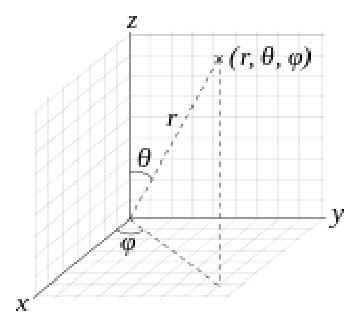
\includegraphics{157px-3D_Spherical.eps} \footnote{\ }

& 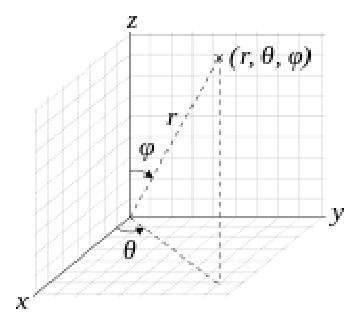
\includegraphics{157px-3D_Spherical_2.eps} \footnote{\ }
\end{tabular}
\end{center}



1-\small{`3D Spherical 2' by Dmcq - Own work. Licensed under Creative Commons Attribution-Share Alike 3.0 via Wikimedia Commons - \href{http://commons.wikimedia.org/wiki/File:3D_Spherical_2.svg\#mediaviewer/File:3D_Spherical_2.svg}{Wikipedia File} } 
\vskip0.1in
2- \small{`3D Spherical' by Andeggs - Own work. Licensed under Public domain via Wikimedia Commons - \href{http://commons.wikimedia.org/wiki/File:3D_Spherical.svg\#mediaviewer/File:3D_Spherical.svg}{Wikipedia File} }
}

\hrule
\vskip0.1in

\begin{problem} 
\marginpar{
	\thomasee{See page 893.} 
	\stewarts{See pages 827-833} 
	\larsonfive{See Larson 11.7.}
	}%
Let $P=(x,y,z)$ be a point in space. This point lies on a cylinder of radius $r$, where the cylinder has the $z$ axis as its axis of symmetry.  The height of the point is $z$ units up from the $xy$ plane. The point casts a shadow in the $xy$ plane at $Q=(x,y,0)$.  The angle between the ray $\vec{OQ}$ and the $x$-axis is $\theta$. Construct a graph in 3D of this information, and use it to develop the equations for cylindrical coordinates given above.
\end{problem}

\begin{problem}\label{derive spherical coordinates} Let 
\marginpar{
	\thomasee{See page 897.}
	\larsonfive{See Larson 11.7.}
	}% 
  $P=(x,y,z)$ be a point in space. This point lies on a sphere of
  radius $\rho$ (``rho''), where the sphere's center is at the origin
  $O=(0,0,0)$. The point casts a shadow in the $xy$ plane at
  $Q=(x,y,0)$.  The angle between the ray $\vec{OQ}$ and the $x$-axis
  is $\theta$, and is called the azimuth angle. The angle between
  the ray $\vec{OP}$ and the $z$ axis is $\phi$ (``phi''), and is
  called the inclination angle, polar angle, or zenith angle.  Construct
  a graph in 3D of this information, and use it to develop the
  equations for spherical coordinates given above.
\end{problem}

\marginpar{See the
  \href{http://en.wikipedia.org/wiki/Spherical_coordinate_system}{Wikipedia}
  or
  \href{http://mathworld.wolfram.com/SphericalCoordinates.html}{MathWorld}
  for a discussion of conventions in different disciplines.}%
	
There is some disagreement between different fields about the notation
for spherical coordinates.  In some fields (like physics), $\phi$
represents the azimuth angle and $\theta$ represents the inclination
angle.  In some fields, like geography, instead of the inclination angle, the
\emph{elevation} angle is given---the angle from the $xy$-plane (lines
of lattitude are from the elevation angle).
Additionally, sometimes the coordinates are written in a different
order.  You should always check the notation for spherical coordinates
before communicating using them.
\vskip0.1in
\hrule
\vskip0.1in
\noindent \Large After Class: \normalsize

\begin{problem}
For each curve below, set up an integral formula which would give the length, and sketch the curve. Do not worry about integrating them.  \marginpar{The reason I don't want you to actually compute the integrals is that they will get ugly really fast. Try doing one in Wolfram Alpha and see what the computer gives.}
\begin{enumerate}
\item The parabola $\vec p(t) = (t,t^2)$ for $t\in[0,3]$.
\item The ellipse $\vec e(t) = (4\cos t,5\sin t)$ for $t\in[0,2\pi]$.
\item The hyperbola $\vec h(t) = (\tan t,\sec t)$ for $t\in[-\pi/ 4,\pi/4]$.
\end{enumerate}
\end{problem}
To actually compute the integrals above and find the lengths, we would use a numerical technique to approximate the integral (something akin to adding up the areas of lots and lots of rectangles as you did in first semester calculus).

\valpo{
\begin{problem}
If you have never worked in Maple, you will want to spend some time familiarizing yourself with the program before our Lab day (keep reading if you are!). The link here takes you to a set of modules which will review several of the vector concepts we learned last week, but also introduce you to Maple. The Vector exploration contains a very nice visual on vector projections, which you should look at even if you are comfortable in Maple.
\vskip0.1in
The Connected Curriculum Project:\\
\href{https://www.math.duke.edu/education/ccp/resources/learn/index.html}{Introduction to Modules}
\vskip0.1in
\href{https://www.math.duke.edu/education/ccp/materials/mvcalc/javamaptutor/contents.html}{Maple Tutorial}
\vskip0.1in
\href{https://www.math.duke.edu/education/ccp/materials/mvcalc/vectors/index.html}{Vectors Exploration}
\end{problem}
}


%%% Local Variables: 
%%% mode: latex
%%% TeX-master: "215-problems"
%%% End: 
